Avant de se lancer tête baissée dans une expérience, dans des recherches, ou dans un code, il faut impérativement avoir une idée de ce que l'on veut avoir.
Cela comprend le design, les fonctionnalités, les représentations.

Même si cette première vision est large et peut-être très éloignée du programme que nous obtiendrons au final, il faut se fixer un objectif à atteindre.

Voici un aperçu du programme : 
\begin{figure}[H]
	\begin{center}
	  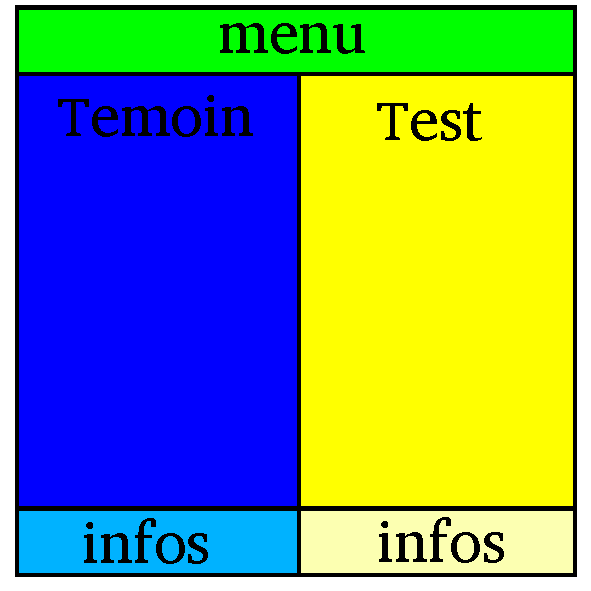
\includegraphics[width=12em]{Images/maquette.pdf}
	\end{center}
	\caption{Une première maquette}
	\label{Maquette}
\end{figure}

Nous avons : 
\begin{description}
	\item[Un menu] qui contrôle les différentes actions
	\item[Deux boites de pétri] qui représentent le témoin et le test
	\item[Une barre d'information] qui affiche les informations relatives aux simulations
\end{description}

C'est fini pour le design, maintenant il faut définir ce qu'on attend de la simulation : 
\begin{itemize}
	\item Des cellules qui se divisent
	\item Des UV qui les tuent / font muter
	\item Ajouter des cellules
	\item Tuer des cellules
	\item Compter les cellules
\end{itemize}

À partir de ces idées nous pouvons avancer vers la réalisation du début de programme qui n'intègre pas encore les valeurs des expériences et recherches. Juste créer le moule qui contiendra le gateau. 




